\section{目的}
2週目の実験では,コンピュータ上で回路図を設計した.しかし大規模な回路の制作に回路図は向いていない.
多くの場合,ハードウェア記述言語 (HDL; Hardware Description Language) を用いて記述される.
3週目は HDL の1種である Verilog を用いて回路設計を行う.
Verilog は C言語と似た言語であり,C言語習得者にとっては感覚的に扱いやすい言語である.

\section{実験方法}

\subsection{課題1 全加算器}
半加算器,全加算器を Verilog で記述する.ただし手続きブロックと算術演算子を用いてはならない.
ここで全加算器は,A, B, $C_I$の入力の和を求める回路である.
全加算器の真理値表を\ref{tab:FA}に示す.

\begin{table}[htb]
  \centering
  \caption{全加算器の真理値表}
  \label{tab:FA}
  \begin{tabular}{ccc|cc}
    $A$ & $B$ & $C_I$ & $C_O$ & $S$ \\ \hline
     0  &  0  &  0  &  0    &  0\\
     0  &  0  &  1  &  0    &  1\\
     0  &  1  &  0  &  0    &  1\\
     0  &  1  &  1  &  1    &  0\\
     1  &  0  &  0  &  0    &  1\\
     1  &  0  &  1  &  1    &  0\\
     1  &  1  &  0  &  1    &  0\\
     1  &  1  &  1  &  1    &  1\\
  \end{tabular}
\end{table}

ソースコードをソースコード\ref{lst:FA-source}に示す.
テストベンチをソースコード\ref{lst:FA-testbench}に示す.


\subsection{課題2について}
課題2は選択問題だが,実験時間が余ったため,両方とも実験を行った.両方ともレポートにまとめておく.

\subsection{課題2A 4ビット加減算器}
4ビット加減算器を作成する.加減算機とは,制御入力の値に応じ,加算器または減算器となる回路である.
減算は,$S=A-B$などという式に対し,2の補数表現を用いて$C = -B = (B \oplus 4'hF) + 1$と変形することで,
$S=A+C$という式で記述することができる.
%
そのため,通常の加算器に対し,XORを通して符号を反転させ,
全加算器の0ビット目のキャリービットを1にすることで,減算器を実現することができる.
図\ref{fig:fa-sign-sch}に回路図を示す.図中,FAは全加算器という意味である.
\begin{figure}[tbp]
  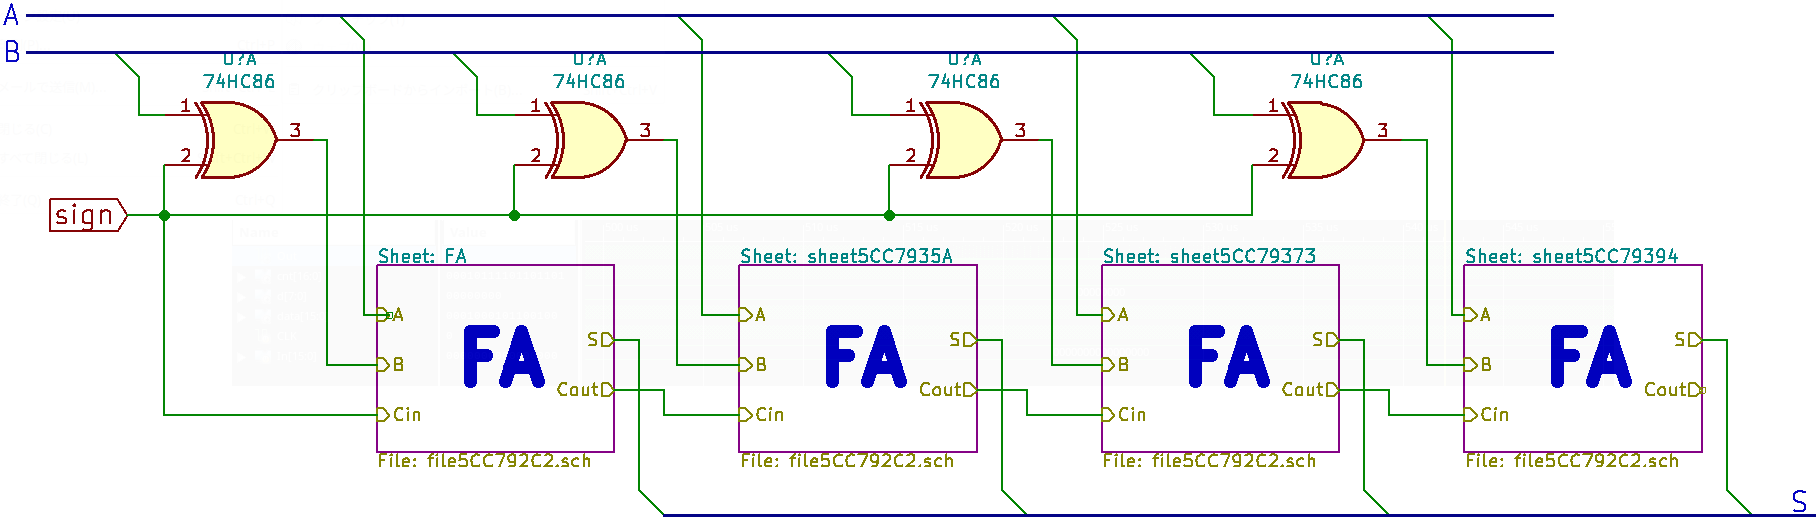
\includegraphics[angle=0,width=160mm]{week3/pics/FA-sign-sch.png}
  \centering
   \caption{加減算器の構成} %タイトルをつける
   \label{fig:fa-sign-sch} %ラベルをつけ図の参照を可能にする
\end{figure}
実際には,最終ビットのキャリービットの出力もモジュールから出力させる.

ソースコードをソースコード\ref{lst:addsub-source}に示す.
テストベンチをソースコード\ref{lst:addsub-testbench}に示す.


\subsection{課題2B 4ビット乗算器}
符号なし4ビット乗算器を制作する.4ビットの掛け算の積は8ビットとなる.
2進数での掛け算は,10進法での筆算と同じように行う(表\ref{tab:binarymult}).

\begin{table}[htb]
  \centering
  \caption{2進法での筆算例}
  \label{tab:binarymult}
  \begin{tabular}{ccccccccc}
     & & & &1&0&1&0&\\
     & & &$\times$&0&1&0&1&\\ \hline
     & & & &1&0&1&0&(1)\\
     & & &0&0&0&0& &(0)\\
     & &1&0&1&0& & &(1)\\
    +&0&0&0&0& & & &(0)\\ \hline
     &0&1&1&0&0&1&0&\\
  \end{tabular}
\end{table}

具体的には,$C=A\times B$の演算に対して,$A$を左にシフトしつつ,$B$の各ビットで全体をマスクし,最後に合算する.
筆算例とHDLで記述されたソースコードを合わせて見ながら理解してもらいたい.
ソースコードをソースコード\ref{lst:handmult-source}に示す.
テストベンチをソースコード\ref{lst:handmult-testbench}に示す.


\subsection{課題3 手続きブロックを用いた7セグメントデコーダの作成}
2週目の課題にあった7セグメントLED用のデコーダを手続きブロックを用いて記述する.
ソースコードをソースコード\ref{lst:block-7segled-source}に示す.
テストベンチをソースコード\ref{lst:block-7segled-testbench}に示す.


\subsection{課題4 7セグメントLEDへの出力と発光の関係の観察}
7セグメントLEDの光り方を調べるため,7セグメントLEDとスイッチをバッファで連結し,光り方を観察する.

ピンの割り当ては,詳細は付録にまとめておく(ソースコード\ref{lst:check-7segled-pinasign}).
ボタンとLEDへの出力の光らせ方も,ソースコード\ref{lst:check-7segled-source}で記述している.

7セグメントLEDはアノードコモンである.
カソード側はAセグメントからG,dotのLEDに繋がっていて,4桁すべて同じ端子を共有している.
プッシュスイッチ側スイッチはプルダウン抵抗を通して何も押されない状態では0出力となる.
IOの割り当てでは,スライドスイッチをLEDのカソード側8ビットに割り当てをした.
プッシュスイッチは,アノード側に4桁分配置した.

7セグメントLEDの光り方を調べる前に期待される動作を考える.
7セグメントLEDのアノード側は Low 状態で光る状態の準備ができる.
カソード側はHigh状態になることで光る準備ができ,
両方が成立したセグメントのLEDが発光することが期待できる.

そのため,まずはプッシュボタンは何も押さず,すべての桁を選択した状態でテストを開始する.
スライドスイッチとLEDの発光の関係を調査する.
その次にスライドスイッチはすべてHighの状態にし,スライドスイッチを1つずつ押して,桁が無効になるかを観察する.

\subsection{課題5 7セグメントLED表示回路の作成}
7セグメントLEDへ実際の数値のの出力をテストする.
押しボタン3つを3ビットの入力とし,それに応じた数字をすべての桁の7セグメントLEDに出力する回路を作成する.

7セグメントLEDとスイッチのピン割り当てをソースコード\ref{lst:check-7segledx1111-pinasign}に示す.
その他の7セグメントLEDの表示ソースコードを\ref{lst:check-7segledx1111-source}に示す.


\subsection{課題6 乗算における符号について}
4ビット乗算器について,符号ありと符号なし両方の演算結果の違いを観測する.
ソースコードをソースコード\ref{lst:multitest-source}に示す.
テストベンチをソースコード\ref{lst:multitest-testbench}に示す.


%% \clearpage
%==============================================
\section{実験結果}
\subsection{課題1 全加算器}
シミュレーション結果の波形を図\ref{fig:adder-sim}に示す.

\begin{figure}[tbp]
  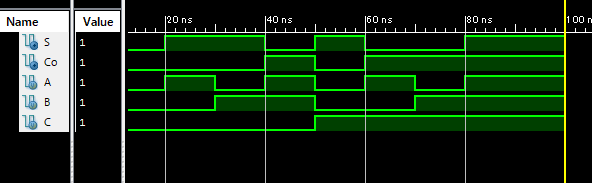
\includegraphics[angle=0,width=140mm]{week3/pics/adder-sim.png}
  \centering
  \caption{全加算器のモジュールテスト} %タイトルをつける
  \label{fig:adder-sim} %ラベルをつけ図の参照を可能にする
\end{figure}


\subsection{課題2A 4ビット加減算器}
Bの符号を正のまま,つまり加算中のシミュレーション結果の1部の波形を図\ref{fig:addersub-add-sim}に示す.
Bの符号を負にし,減算中のシミュレーション結果の1部の波形を図\ref{fig:addersub-sub-sim}に示す.
波形中,SIGNが符号を示しており,すべてのデータは符号ありと仮定して表示している.出力Cは桁溢れを示している.
図中,変数J, K, SIはループ変数で特に意味はない.

\begin{figure}[tbp]
  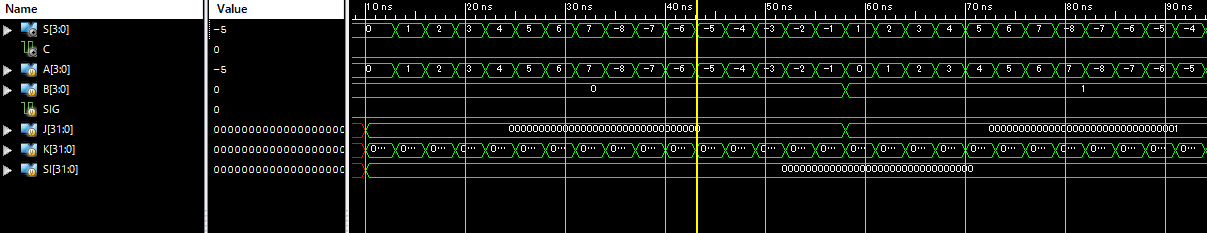
\includegraphics[angle=0,width=160mm]{week3/pics/addersub-add-sim.png}
  \centering
  \caption{加減算器の加算時のモジュールテスト} %タイトルをつける
  \label{fig:addersub-add-sim} %ラベルをつけ図の参照を可能にする
\end{figure}

\begin{figure}[tbp]
  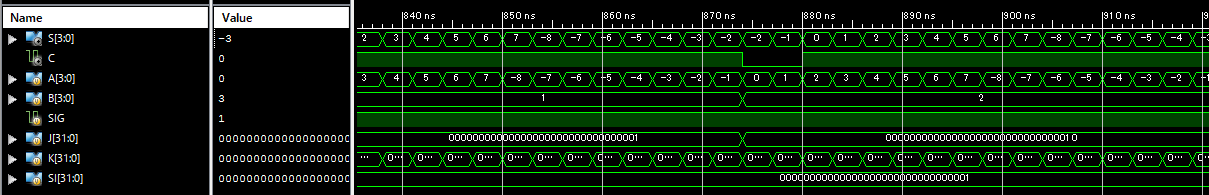
\includegraphics[angle=0,width=160mm]{week3/pics/addersub-sub-sim.png}
  \centering
  \caption{加減算器の減算時のモジュールテスト} %タイトルをつける
  \label{fig:addersub-sub-sim} %ラベルをつけ図の参照を可能にする
\end{figure}


\subsection{課題2B 4ビット乗算器}
4ビット乗算器のモジュールテストの結果の1部を図\ref{fig:handmade-mul-sim}に示す.
図中,変数J, Kはループ変数で特に意味はない.

\begin{figure}[tbp]
  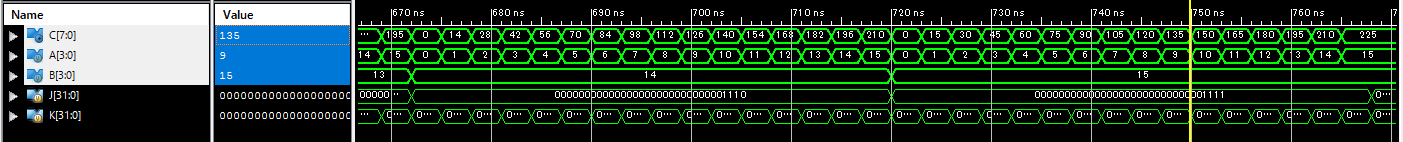
\includegraphics[angle=0,width=160mm]{week3/pics/multi-unsigned-handmade-sim.png}
  \centering
  \caption{4ビット乗算器のモジュールテスト} %タイトルをつける
  \label{fig:handmade-mul-sim} %ラベルをつけ図の参照を可能にする
\end{figure}

\subsection{課題3 手続きブロックを用いた7セグメントデコーダの作成}
7セグデコーダのモジュールテストの結果を図\ref{fig:decode7seg-block}に示す.
2週目の課題同様に赤の線に注目するとデコード結果が見える.
\begin{figure}[tbp]
  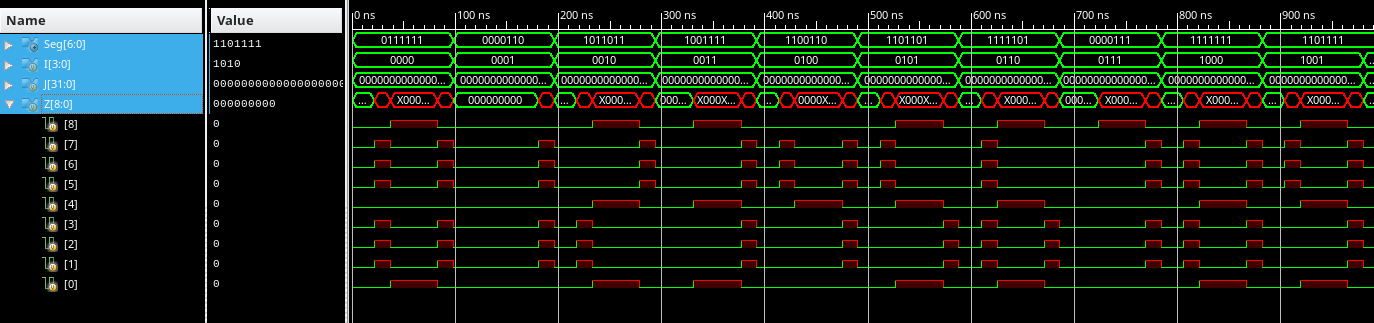
\includegraphics[angle=0,width=160mm]{week3/pics/7seg-dec-sim.png}
  \centering
  \caption{7セグデコーダのモジュールテスト} %タイトルをつける
  \label{fig:decode7seg-block} %ラベルをつけ図の参照を可能にする
\end{figure}

\subsection{課題4 7セグメントLEDへの出力と発光の関係の観察}
出力値と7セグメントLEDの光り方の調査結果を調べた.
実験方法で述べたように,課題4の実験は2つに分けて行われた.

前者のほうでは,プッシュスイッチを押さずにセグメントの発光パターンを調査する.
結果としては,割り当てたセグメントとスライドスイッチの間の関係性が検証できた.
dotに関してはHigh出力のとき,小数点を表現するときに用いられる''.''が現れた.
その他,回路図のセグメントの割り当てと同じようにセグメントがHighで点灯した.

次に後者の方では,スライドスイッチを幾つかHighにセットした状態で1つずつプッシュスイッチを押す.
押すとスイッチの出力はHighになる.
押した桁に対応する桁が消灯した.
4つ全て押すと完全に消灯した.
3つだけ押すと,一つだけ残して消えた.

\subsection{課題5 7セグメントLED表示回路の作成}
7セグメントLEDは目的の動作を果たしていた.0-7のバイナリ入力に対応する7セグメント表示ができていた.

\subsection{課題6 乗算における符号について}
テストベンチの結果を図\ref{fig:mult-sighned-unsigned}に示す.符号を考慮した演算結果になっている.
符号なしでは単に乗算計算をしている.

\section{考察}
\subsection{課題1 全加算器}
1ビットの加算計算ができていることがわかる.

\subsection{課題2A 4ビット加減算器}
4ビットの加減算計算が正しく動作していることがわかる.

\subsection{課題2B 4ビット乗算器}
4ビットの乗算計算が正しく動作していることがわかる.
符号は考慮していないので,符号なしの計算のみしかできない.

\subsection{課題3 手続きブロックを用いた7セグメントデコーダの作成}
7セグメントLED用のデコードが正しく動作していることがわかる.
2週目で設計した回路図と同様の動作をした.
こちらのほうが開発時間がかなり短くなっている.
以前は3時間くらいはかかってたが,今回は20分くらいで同様の動作を実現した.

\subsection{課題4 7セグメントLEDへの出力と発光の関係の観察}
7セグメントLEDの動作として,桁を決めるピンと,7セグメントLEDのセグを制御するポートがあることがわかる.
ポートとセグメントの対応は,回路図通りであることが分かった.
アノード側はLowで光ることがわかる.
カソード側はHighで光る.

両方がANDの条件式になっていて,両方成り立つときのみLEDが点灯する.
セグメントの制御用ポートがすべての桁で共通していることから,
すべての桁を別々に,また同時に制御することはできない.
桁を高速に切り替えながら,それぞれの桁を表示するダイナミック制御を行うことが考えらる.

4桁の7セグメントLEDのように,なにも工夫しないと$(7+1)\times4=32$個のLEDを同時に制御するのには多数のポートが必要になる.
しかしFPGAではポートが有限であるため,1つのLEDに1つのポートを対応させるのは入出力ポートの資源の面から考えると良くない.
この回路で使われているダイナミック点灯の方式では,この場合は$8+4=12$ポートで制御できる.
半分以下までポート数を削減できるが,同時には制御できないので,高速に桁を切り替えながら表示することが考えられる.
そのためデメリットとしてはLEDの輝度が$\frac{1}{4}$まで低下することが考えられる.

\subsection{課題5 7セグメントLED表示回路の作成}
7セグメントLED用の出力を正しく動作している.
今回はcase文で実装しているが,if文でも同様の実装ができることが考えられる.

\subsection{課題6 乗算における符号について}
符号ありと符号なしの乗算の演算結果に違いが出た.
符号ありでは,私たちは普段,符号同士の演算を別にしておいて,後で符号をまとめる.
乗算器でも同様に,符号なしでは符号の計算は考慮されなかった.
すべて符号なしとして処理されている.
逆に符号ありでは,符号を考慮しての計算ができていることがわかる.

\begin{figure}[tbp]
  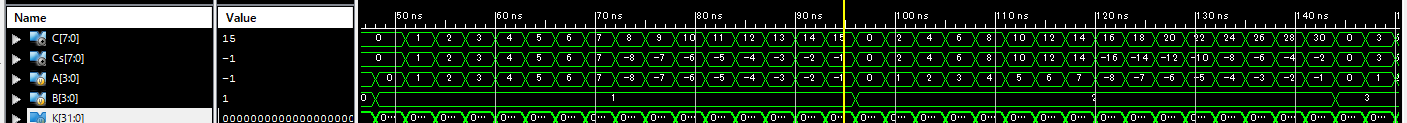
\includegraphics[angle=0,width=160mm]{week3/pics/multi-signed-unsigned.png}
  \centering
  \caption{4ビット乗算器における符号ありと符号なしの違い} %タイトルをつける
  \label{fig:mult-sighned-unsigned} %ラベルをつけ図の参照を可能にする
\end{figure}

\section{感想}
以前7セグメントLED用のデコード回路を作成したときよりもVerilogで記述したほうが製作時間が短くった.
ハードウェアの最適化は人がやるところと機械に任せるところの選定が必要だと思った.
全体の構造は人の手で決めるべきだが,細かい部分はコンピュータの論理合成により行われたほうが簡単にできる.

また,7セグメントLEDの制御回路に工夫が見られた.
ポート数は,マイコンでプログラミングする際にも制約として考慮しなければならないことが多い.
少ないポートで効率よく制御するためには,回路上の工夫が欠かせないことがわかった.

また,加算器に関しては,このままでは桁が長くなると,計算時間が長くなると思った.
桁上がりが入るのが,前の桁を計算しなければ桁上がりがわからないためである.
高速化するには桁上がりを前もって計算するための機構などを用意する必要があると思う.


\clearpage
\section{付録}
\lstinputlisting[caption=課題1 ソースコード,label=lst:FA-source]{week3/source/adder.v}
\lstinputlisting[caption=課題1 テストベンチ,label=lst:FA-testbench]{week3/source/addertestbench.v}

\lstinputlisting[caption=課題2A ソースコード,label=lst:addsub-source]{week3/source/addsub4.v}
\lstinputlisting[caption=課題2A テストベンチ,label=lst:addsub-testbench]{week3/source/addsub4testbench.v}

\lstinputlisting[caption=課題2B ソースコード,label=lst:handmult-source]{week3/source/handmulti.v}
\lstinputlisting[caption=課題2B テストベンチ,label=lst:handmult-testbench]{week3/source/handmulti-testbench.v}

\lstinputlisting[caption=課題3 ソースコード,label=lst:block-7segled-source]{week3/source/seg7decblock.v}
\lstinputlisting[caption=課題3 テストベンチ,label=lst:block-7segled-testbench]{week3/source/7segtestbench.v}

\lstinputlisting[caption=課題4 ピン割り当て,label=lst:check-7segled-pinasign]{week3/source/check7seg.ucf}
\lstinputlisting[caption=課題4 ソースコード,label=lst:check-7segled-source]{week3/source/check7seg.v}

\lstinputlisting[caption=課題5 ピン割り当て,label=lst:check-7segledx1111-pinasign]{week3/source/seg7proc.ucf}
\lstinputlisting[caption=課題5 ソースコード,label=lst:check-7segledx1111-source]{week3/source/seg7proc.v}

\lstinputlisting[caption=課題6 ソースコード,label=lst:multitest-source]{week3/source/multitest.v}
\lstinputlisting[caption=課題6 テストベンチ,label=lst:multitest-testbench]{week3/source/multitesttestbench.v}
